% ============================================================================
\section{Supplementary Tables, Derivations, and Evaluation Details}
% ============================================================================

\subsection{Notation and experimental configurations}
\label{app:reference_tables}

\begin{table}[H]
\centering
\small
\caption{Notation and the four-teacher configuration.}
\label{tab:notation}
\begin{tabular}{cll}
\toprule
Symbol & Meaning & Value in this study \\
\midrule
$M$ & number of tasks and teachers & $4$ \\
$w_i$ & fixed objective weight & inverse initial loss, normalized \\
$G$ & micro-batches per optimizer step & $16$ \\
$b$ & prompts per micro-batch; one response each & $4$ \\
$m_i$ & task-$i$ micro-batch count & $2\leq m_i\leq8$ \\
$g_{i,s}$ & unweighted micro-batch gradient & measured during backward \\
$D$ & AdamW diagonal scaling & $(\sqrt v+\epsilon)^{-1}$ \\
$e_i$ & one-micro-batch noise after scaling by $D$ & estimated each step \\
$\tau_i,C$ & marginal task time; fixed step overhead & timing averages \\
$H$ & variance ratio relative to Uniform & $H\leq2$ from the count bound \\
\bottomrule
\end{tabular}
\end{table}

\begin{table}[H]
\centering
\footnotesize
\caption{Four-teacher MOPD configuration.}
\label{tab:pipeline}
\begin{tabular}{p{0.20\linewidth}p{0.72\linewidth}}
\toprule
Component & Configuration \\
\midrule
Student & Qwen3-1.7B \citep{qwen2025qwen3};
\missing{exact checkpoint revision; Base/SFT/Instruct status; initial scores} \\
Teachers & One fixed specialist for each of math, code, instruction following,
and science; \missing{teacher names, sizes, revisions, origins, and same-origin
status} \\
Training prompts & $16{,}000$ unique prompts per task, shuffled once and read
without replacement; \missing{dataset names, versions, licenses, and filters} \\
Rollout and loss & One response per prompt; one update per rollout batch
($K=1$); sampled-token reverse KL, averaged over valid tokens and then prompts;
maximum response length $8{,}192$; \missing{temperature, ratio-truncation rule,
and observed truncation rate by task} \\
Step and budget & $b=4$ prompts per micro-batch, $G=16$ micro-batches per step,
$500$ steps, and $32{,}000$ attempted responses; $2\leq m_i\leq8$ \\
Optimization & AdamW; inverse-initial-loss objective weights fixed before
training; \missing{learning rate and schedule, $\beta_1$, $\beta_2$, $\epsilon$,
weight decay, gradient clipping, precision, and sharding} \\
System & At most one teacher loaded at a time, in a fixed cyclic order;
\missing{GPU type and count, inference engine, software revisions, and GPU hours
per run} \\
\bottomrule
\end{tabular}
\end{table}

\begin{table}[H]
\centering
\small
\caption{Training configurations. ``Conv.'' denotes conventional AdamW and
``TW'' the optional observation in Equation~\ref{eq:taskwise_square_observation}.}
\label{tab:exp_methods}
\begin{tabular}{lll}
\toprule
Configuration & Count rule & AdamW second moment \\
\midrule
Uniform & $(4,4,4,4)$ & Conv. \\
GPAS & $w_i\sqrt{e_i}$ & Conv. \\
Cost-GPAS & integer minimizer of Equation~\ref{eq:batch_cost_objective} & Conv. \\
RawNoise & $w_i\sqrt{\operatorname{Var}(g_i)}$ & Conv. \\
Uniform--TW & $(4,4,4,4)$ & TW \\
GPAS--TW & $w_i\sqrt{e_i}$ & TW \\
\bottomrule
\end{tabular}
\end{table}

\subsection{One-step variance criterion}
\label{app:descent}

Let $D$ be fixed within the step. If $F$ is $L$-smooth and
$\theta'=\theta-\eta DA$, then
\begin{equation}
    \mathbb E[F(\theta')]
    \leq F(\theta)-\eta\nabla F^\top D\nabla F
    +\frac{\eta^2L}{2}
      \left(\|D\nabla F\|_2^2+V(m)\right).
    \label{eq:one_step_descent}
\end{equation}
For a fixed student state, $D$, and step size, only $V(m)$ depends on the
allocation. This local calculation motivates the variance criterion; the
end-to-end experiment includes momentum and gradient clipping.

\subsection{Fixed objective and taskwise second-moment scale}
\label{app:moment_target_proof}

For a fixed allocation, assume task-$i$ micro-batch gradients are independent
with mean $h_i$ and coordinatewise variance $\sigma_i^2$. Equation
\ref{eq:batch_gradient_observation} gives
\begin{equation}
    \mathbb E[A]=\sum_iw_i h_i,
    \qquad
    \mathbb E[A^2]=\left(\sum_iw_i h_i\right)^2
    +\sum_i\frac{w_i^2}{m_i}\sigma_i^2.
    \label{eq:conventional_batch_second_moment}
\end{equation}
Thus the conventional AdamW second-moment observation has an
allocation-dependent noise term. For the taskwise observation,
\begin{equation}
    \mathbb E[U/G]
    =\frac{1}{G}\sum_iw_i\left(h_i^2+\sigma_i^2\right),
    \label{eq:consistent_second_moment_target}
\end{equation}
which is independent of $m$. At proportional allocation $m_i=Gw_i$, the noise
term in Equation~\ref{eq:conventional_batch_second_moment} is exactly
$G^{-1}\sum_iw_i\sigma_i^2$, matching Equation
\ref{eq:consistent_second_moment_target}. The signal terms remain different:
conventional AdamW uses $(\sum_iw_i h_i)^2$, whereas TW uses
$G^{-1}\sum_iw_i h_i^2$. In noise-dominated coordinates, using $U$ without the
$1/G$ factor would enlarge the second-moment target by about $G$ and shrink
updates by about $\sqrt G$; the main implementation therefore uses $U/G$.

\subsection{Gradient variance and its within-step estimate}
\label{app:variance}

Independence across tasks and micro-batches gives
\begin{align}
\mathbb E\|D(A-\mathbb E[A])\|_2^2
&=\sum_iw_i^2\mathbb E\|D(\bar g_i-h_i)\|_2^2 \\
&=\sum_i\frac{w_i^2}{m_i}
  \mathbb E\|D(g_i-h_i)\|_2^2,
\end{align}
which is Equation~\ref{eq:batch_variance}. For one task,
\begin{equation}
\sum_{s=1}^{m_i}\|D(g_{i,s}-\bar g_i)\|_2^2
=\sum_{s=1}^{m_i}\|Dg_{i,s}\|_2^2-m_i\|D\bar g_i\|_2^2.
\end{equation}
Dividing by $m_i-1$ gives the standard unbiased sample-variance estimate summed
over AdamW-scaled coordinates. It is defined whenever $m_i\geq2$.

\subsection{Variance and cost allocations}
\label{app:allocation_proofs}

Write $q_i=w_i\sqrt{e_i}$. With equal micro-batch cost,
\begin{equation}
\left(\sum_i m_i\right)\left(\sum_i\frac{q_i^2}{m_i}\right)
\geq\left(\sum_i q_i\right)^2.
\end{equation}
Equality holds at $m_i\propto q_i$, giving GPAS. With task-dependent cost and
zero fixed overhead,
\begin{equation}
\left(\sum_i m_i\tau_i\right)
\left(\sum_i\frac{q_i^2}{m_i}\right)
\geq\left(\sum_i q_i\sqrt{\tau_i}\right)^2,
\end{equation}
with equality at $m_i\propto q_i/\sqrt{\tau_i}$. For $C>0$, Cost-GPAS evaluates
the full objective in Equation~\ref{eq:batch_cost_objective} over feasible
integer counts.

\subsection{Controlled calculation and estimator checks}
\label{app:controlled}

The controlled check uses three Gaussian micro-batch gradients in three
coordinates and a diagonal AdamW scaling that changes their noise ranking.
Every step contains $G=16$ micro-batches with $2\leq m_i\leq12$. Bounded
rounding gives counts $(6,5,5)$ for Uniform, $(11,3,2)$ for RawNoise,
$(3,3,10)$ for GPAS, and $(3,5,8)$ for zero-overhead Cost-GPAS. All methods use
the same fixed weights and common random numbers over $20{,}000$ trials.

\begin{figure}[H]
    \centering
    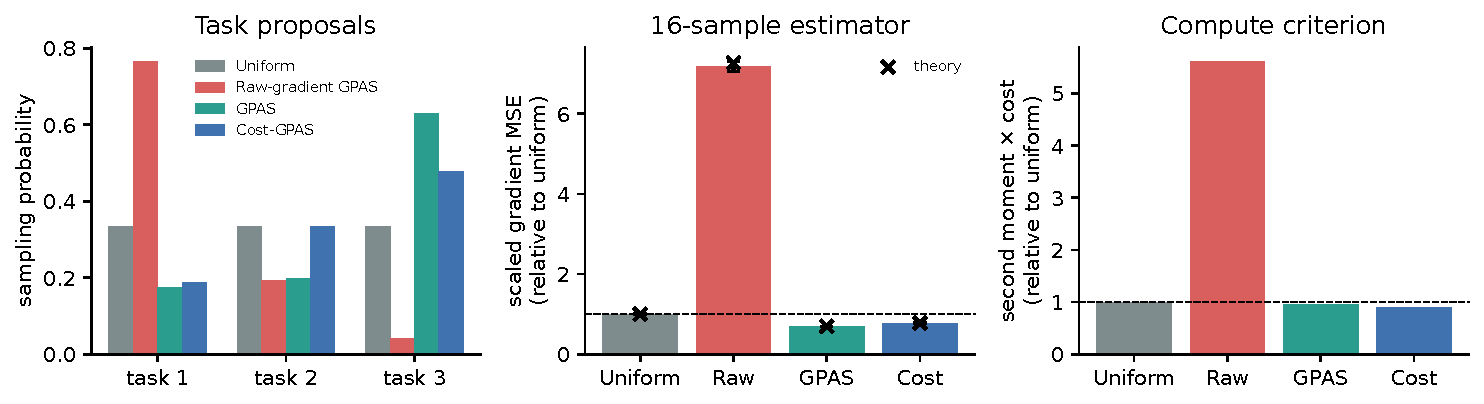
\includegraphics[width=0.98\linewidth]{figures/controlled_optimizer_sampling.pdf}
    \caption{Controlled checks. Bars are Monte Carlo estimates and crosses are
    calculated values. GPAS uses AdamW-scaled within-task noise; Cost-GPAS also
    uses task cost. The last panel compares second-moment observations after an
    integer reallocation.}
    \label{fig:controlled_checks}
\end{figure}

Over $200{,}000$ simulated steps, reallocating from Uniform to GPAS changes the
conventional $A^2$ observation by $0.543$ in relative norm, compared with
$0.542$ from Equation~\ref{eq:conventional_batch_second_moment}. The taskwise
$U/G$ observation changes by $0.00092$ from Monte Carlo error; its theoretical
target is unchanged.

At early, middle, and late Uniform checkpoints, the held-out variance check
splits each task's fixed micro-batch set in half. Each half estimates
$\widehat e_i$ and an allocation, which are evaluated on the other half, and
then the roles are exchanged. \missing{Insert held-out estimator error and
variance ratios after collecting the checkpoint gradients.}

\subsection{MOPD loss and micro-batch normalization}
\label{app:opd_estimators}

For a student-generated prefix $z$, write
$q_v=\pi_\theta(v\mid z)$ and $t_v=T_i(v\mid z)$. The sampled-token reverse-KL
score is
\begin{equation}
    \operatorname{sg}\!\left[\log\frac{q_V}{t_V}\right]
    \nabla_\theta\log q_V,\qquad V\sim q.
\end{equation}
The implementation averages valid tokens within one response and then the
$b=4$ responses from distinct prompts in a micro-batch. Any configured
importance-ratio truncation is applied before these means; the fixed-objective
factor $w_i/m_i$ is applied after them. There is no groupwise advantage
normalization and no outcome-reward term.

\subsection{System timing, logs, and resume tests}
\label{app:system_details}

For each task in a step, the log records teacher load and offload time,
teacher-ready time, rollout, scoring, backward, optimizer time, peak HBM,
attempted responses, valid tokens, and generated tokens. Unhidden transfer time
is the positive difference between teacher-ready time and rollout-end time. GPU
hours include all model-transfer and waiting time. The fitted fixed overhead is
the remaining step time after subtracting the marginal per-micro-batch times.

Checkpoints store the current allocation, noise values, timing averages,
rounding state, prompt positions, and AdamW variant. A resume test reproduces
the next allocation, moment observations, and parameter update. Generated
tokens per micro-batch provide an alternative cost measure when detailed event
timing is unavailable. Under ideal concurrent teacher execution, the time model would
be $C+\max_i m_i\tau_i$ rather than the serial sum, so only the fixed-objective
scaling and GPAS rule transfer unchanged.

\subsection{Full task-level trajectories}

\begin{figure}[H]
    \centering
    \missingfigure[0.18\textheight]{Insert all per-task teacher-loss curves,
    prompt consumption, response length and truncation trajectories, count-bound
    occupancy, and step-time quantiles from the released logs.}
    \caption{Task-level training and system traces.
    \missing{Replace after the four-teacher runs finish.}}
    \label{fig:appendix_task_curves}
\end{figure}
